\documentclass[twocolumn,10pt]{article}

% ==============================================================================
% CSE200 LAB EVALUATION / ONLINE SPEED TEMPLATE
% Designed for 40-45 minute timed write-ups
% ==============================================================================

% ---- Page Layout & Geometry ----
\usepackage[a4paper, margin=1in]{geometry}
\usepackage{float}
\usepackage{wrapfig}
\usepackage{verbatim}
\usepackage{refcount}
% ---- Multi-column Text ----
\usepackage{multicol}

% ---- Colors ----
\usepackage[table,dvipsnames]{xcolor}
\definecolor{customblue}{RGB}{0, 76, 153}
\definecolor{softgreen}{RGB}{226, 245, 236}
\definecolor{softred}{RGB}{255, 232, 232}
\definecolor{softyellow}{RGB}{255, 247, 214}
\definecolor{codegreen}{rgb}{0,0.6,0}
\definecolor{codegray}{rgb}{0.5,0.5,0.5}
\definecolor{codepurple}{rgb}{0.58,0,0.82}
\definecolor{backcolour}{rgb}{0.95,0.95,0.92}

% ---- Graphics & Subfigures ----
\usepackage{graphicx}
\usepackage{caption}
\usepackage{subcaption}

% ---- Tables ----
\usepackage{booktabs}
\usepackage{array}
\usepackage{multirow}

% ---- Lists ----
\usepackage{enumitem}

% ---- Math & Theorems ----
\usepackage{amsmath, amssymb, amsfonts}
\usepackage{amsthm}
\DeclareMathOperator*{\argmax}{arg\,max}
\DeclareMathOperator*{\argmin}{arg\,min}
\newtheorem{proposition}{Proposition}
\newtheorem{theorem}{Theorem}
\newtheorem{lemma}{Lemma}
\newtheorem{corollary}{Corollary}

% ---- Algorithms & Pseudocode ----
\usepackage{algorithm}
\usepackage{algpseudocode}

% ---- Code Listings ----
\usepackage{listings}
\lstdefinestyle{mystyle}{
    backgroundcolor=\color{backcolour},
    commentstyle=\color{codegreen},
    keywordstyle=\color{customblue}\bfseries,
    numberstyle=\tiny\color{codegray},
    stringstyle=\color{codepurple},
    basicstyle=\ttfamily\footnotesize,
    breakatwhitespace=false,
    breaklines=true,
    captionpos=b,
    keepspaces=true,
    numbers=left,
    numbersep=5pt,
    showspaces=false,
    showstringspaces=false,
    showtabs=false,
    tabsize=2,
    frame=single,
    columns=fullflexible,
    linewidth=\textwidth
}
\lstset{style=mystyle}

% ---- Author Affiliations ----
\usepackage{authblk}

% ==============================================================================
% BIBLIOGRAPHY CONFIGURATION (CHOOSE ONE APPROACH)
% ==============================================================================
% --- Approach A: Modern BibLaTeX + Biber (DEFAULT) ---
% Note: Use \textcite{key} for Author (Year) and \parencite{key} for (Author, Year)
\usepackage[backend=biber, style=numeric]{biblatex}
\addbibresource{riemann_hypothesis_refs.bib} % Must include .bib extension!

% --- Approach B: Traditional Natbib / BibTeX ---
% To use Natbib: Uncomment natbib line below AND comment out BibLaTeX lines above!
% Also switch bottom bibliography command from \printbibliography to \bibliography{solar_system}
%\usepackage[numbers, sort&compress]{natbib}
%\usepackage[authoryear, round]{natbib} % For Author-Year style


% ---- Hyperlinks (Load after bib/font packages) ----
\usepackage[colorlinks=true, linkcolor=customblue, citecolor=teal, urlcolor=teal]{hyperref}
% \newtheorem{theorem}{Theorem}
% ==============================================================================
% SPEED MACROS & SHORTCUTS FOR TIMED EVALUATION
% ==============================================================================

% --- Equation Shortcuts ---
\newcommand{\be}{\begin{equation}}
\newcommand{\ee}{\end{equation}}
\newcommand{\bea}{\begin{align}}
\newcommand{\eea}{\end{align}}
% --- Calculus & Derivatives ---
\newcommand{\ddt}[1]{\frac{\mathrm{d}#1}{\mathrm{d}t}}
\newcommand{\ddx}[1]{\frac{\mathrm{d}#1}{\mathrm{d}x}}
\newcommand{\pdt}[1]{\frac{\partial #1}{\partial t}}
\newcommand{\pdx}[1]{\frac{\partial #1}{\partial x}}

% --- Number Sets ---
\newcommand{\R}{\mathbb{R}}
\newcommand{\N}{\mathbb{N}}
\newcommand{\Z}{\mathbb{Z}}
\newcommand{\C}{\mathbb{C}}

% --- Linear Algebra & Vector Notation ---
\newcommand{\vct}[1]{\mathbf{#1}}                % Vector: \vct{x}
\newcommand{\mat}[1]{\mathbf{#1}}                % Matrix: \mat{A}
\newcommand{\I}{\mathbf{I}}                      % Identity Matrix: \I
\newcommand{\zero}{\mathbf{0}}                   % Zero Vector: \zero
\newcommand{\T}{^{\mathsf{T}}}                   % Transpose: A\T
\newcommand{\norm}[1]{\left\lVert #1 \right\rVert}
\newcommand{\abs}[1]{\left| #1 \right|}
\newcommand{\inner}[2]{\langle #1,\, #2 \rangle}
\newcommand{\tr}{\operatorname{tr}}              % Trace
\newcommand{\Real}{\text{Re}}
% --- Probability & Statistics ---
\newcommand{\E}{\mathbb{E}}                      % Expectation: \E[X]
\newcommand{\Var}{\operatorname{Var}}            % Variance
\newcommand{\Cov}{\operatorname{Cov}}            % Covariance
\newcommand{\Prob}{\mathbb{P}}                   % Probability

% --- Computer Science & Algorithms ---
\newcommand{\BigO}[1]{\mathcal{O}\left( #1 \right)}     % Big-O notation: \BigO{n \log n}
\newcommand{\ThetaO}[1]{\Theta\left( #1 \right)}       % Theta notation
\newcommand{\OmegaO}[1]{\Omega\left( #1 \right)}       % Omega notation
\newcommand{\floor}[1]{\left\lfloor #1 \right\rfloor}   % Floor
\newcommand{\ceil}[1]{\left\lceil #1 \right\rceil}     % Ceiling

% --- Text Shortcuts ---
\newcommand{\eg}{\textit{e.g.,}\ }
\newcommand{\ie}{\textit{i.e.,}\ }
\newcommand{\etal}{\textit{et al.}}

% --- Colored Text Shortcuts ---
\newcommand{\blue}[1]{\textcolor{customblue}{#1}}
\newcommand{\red}[1]{\textcolor{red}{#1}}
\newcommand{\warn}[1]{\textcolor{red}{\textbf{WARNING: #1}}}

% Redefine the contents name to include a color
\renewcommand{\contentsname}{\textcolor{blue}{Contents}}


% ==============================================================================
% DOCUMENT BEGINS
% ==============================================================================
\begin{document}

% --- Title Block ---
\title{The Riemann Hypothesis}

\author[$\mp$]{Count Binface}
% \author[2]{Co-Author Name}

\affil[$\mp$]{Leader of Recyclon, Sigma IX \& Master of \LaTeX}
% \affil[2]{Department of Electrical Engineering, BUET}

\date{\today}
\maketitle
\onecolumn
\tableofcontents

% \twocolumn[
% \tableofcontents
% \vspace{1em}
% ]
\clearpage
\twocolumn
\section{A Function built from integers}
\subsection{The Riemann Zeta Function}

For a complex number $s= \sigma+it$ with $\sigma >1$, the Riemann
zeta function is
\begin{equation}
    \zeta(s) = \sum_{n=1}^{\infty} = \prod_{p \text{ prime}} \left( 1-\frac{1}{p} \right) ^{-1}
    \label{eq:one}
\end{equation}
The sum–product identity is the Euler product
and links $\zeta(s)$ with primes \cite{edwards1974}. See the \href{https://www.claymath.org/millennium/riemann-hypothesis/}{Clay Mathematics Institute}\footnote{The Riemann Hypothesis is a Millennium Prize Problem.}

\subsection{A classical special value}
At $s=2$ , Eequation~\ref{eq:one} gives the calssical ifdentity
\begin{align*}
    \zeta(2) &= 1 + \frac{1}{2^2} + \frac{1}{3^2} + \frac{1}{4^2} + \dots = \frac{\pi^2}{6} \\
    \prod_{p\in\{2,3,5,7\}} (1-\frac{1}{p^2})^{-1} &\approx 1.595 < \frac{\pi^2}{6} \approx 1.645.
\end{align*}
More prime factors improve the approximation.

\subsection{Two Mathematical Worlds}
Figure~\ref{fig:one} connects zeta zeros with prime distibution.
\begin{figure*}{H}
    \centering
    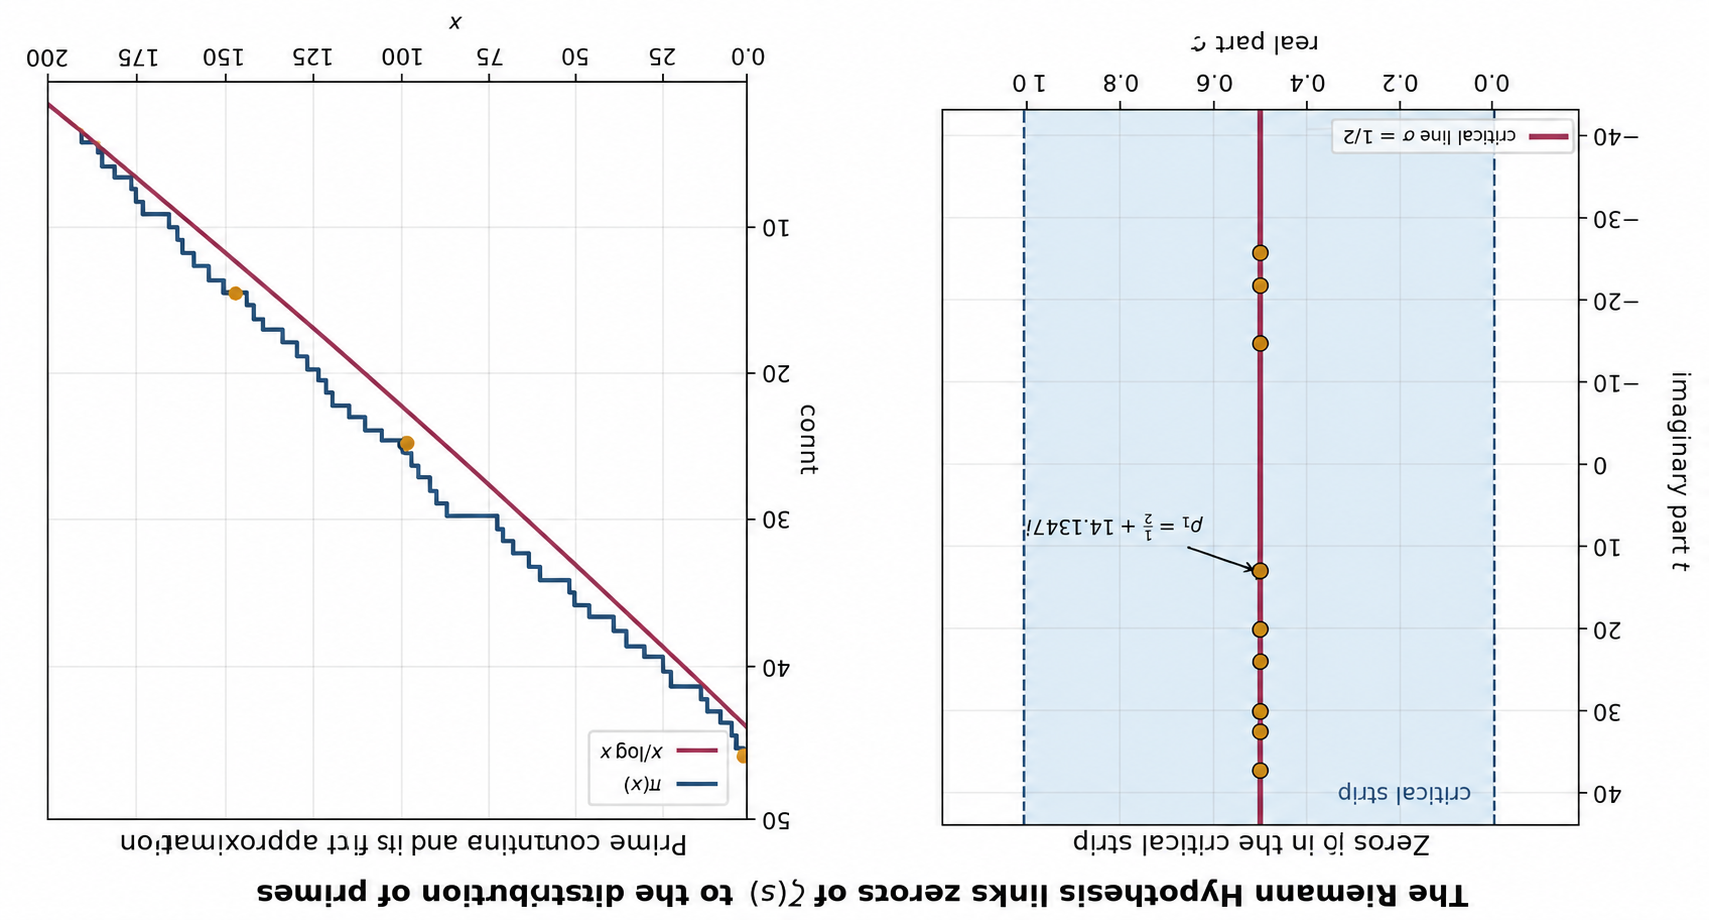
\includegraphics[width=0.9\linewidth, angle=180]{riemann_critical_strip.png}
    \caption{The critical strip and the relation between prime counting and analytic approximation.}
    \label{fig:one}
\end{figure*}
\section{Zeros, Symmetry, and the Critical Line}
\subsection{Trivial and Nonttrivial zeros}
The \emph{trivial zeros} are 
\[-2, -4, -6\]
and the \emph{non trivial zeros} lie in the \emph{cirtical strip}
\[0<\text{Re}(s) < 1\]

\begin{enumerate}[label=\Alph*]
    \item \textbf{Trivial Zeros}
        \begin{itemize}[label=$\nmid$]
            \item They occur at negative even integers.
            \item Their locations are completely understood.
        \end{itemize}
    \item \textbf{Nontrivial zeros}
        \begin{itemize}[label=$\ni$]
            \item  They lie inside the critical strip.
            \item They occur in symmetric families.
            \item Their symmetries generate the following companion points:
            \begin{itemize}[label=\Roman*]
                \item $\rho$
                \item $1-\rho$
                \item $\overline{\rho}$
                \item $1- \overline{\rho}$
            \end{itemize}
            \item Their horizontal locations are central to the Riemann Hypothesis.
        \end{itemize}
\end{enumerate}
\subsection{The funcitonal equation}
A symmetric form of the zeta function is
\begin{equation}
    \zeta(s) = \frac{1}{2}s(s-1)\pi^{-s/2}\Gamma\left(\frac{s}{2}\right)\zeta(s), \quad \zeta(s) = \zeta(1-s)
    \label{eq:two}
\end{equation}
Equation~\ref{eq:two} reflects zeros across $\sigma = 1/2$:
\[
\begin{bmatrix}
    \sigma'\\
    t'
\end{bmatrix} = \begin{bmatrix}
    -1 & 0\\
    0 & 1
\end{bmatrix}\begin{bmatrix}
    \sigma\\
    t
\end{bmatrix} + \begin{bmatrix}
    1\\
    0
\end{bmatrix}
\]
The lineasr part of the reflection is the matris
\begin{equation}
    R = \begin{bmatrix}
    -1 & 0\\
    0 & 1
\end{bmatrix}, \quad R^2 = \begin{bmatrix}
    1 & 0\\
    0 & 1
\end{bmatrix}=I_2
\end{equation}
Hence $R$ is an involution.
\subsection{The first few zeros}
The line $\Real(s) = \frac{1}{2}$ is the \emph{critical line}

\begin{table}[H]
    \centering
    %\rowcolors{2}{blue!20!white}{gray!20}
    \begin{tabular}{|c|c|c|c|}
        \rowcolor{Blue!50} Index & $\gamma_n$ & real part & imaginary part \\
        1 & 14.134725 & \multirow[c]{4}{*}{\textcolor{black}{$\dfrac{1}{2}$}} & 14.134725 \\
        2 & 21.022040 & & 21.022040 \\
        3 & 25.010858 & & 25.010858 \\
        4 & 30.424876 & & 30.424876 \\
        \bottomrule
    \end{tabular}
    \caption{ The first four positive ordinates of nontrivial zeros.}
    \label{tab:one}
\end{table}
The first two zeros form the matrix


\begin{equation}
Z = \begin{bmatrix}
    \frac{1}{2} & 14.134725 \\
    \frac{1}{2} & 21.022040
    \end{bmatrix}
\end{equation}
Each row stores one zero.
\subsection{A Numerical Inspection Procedure}
Algorithm~\ref{alg:one}
test candiate reak part
\begin{algorithm}[H]
    \caption{ Check candidate zeros against the critical line}
    \label{alg:one}
    \begin{algorithmic}[1]
        \Require Candidate zeros $Z=(\rho_1, \rho_2, \ldots , \rho_M$ and tolerance $\varepsilon > 0$
        \Ensure \textsc{True} if every candiate satisfies $|\Real(\rho_i) - \frac{1}{2}| \le \varepsilon$
        \State $allOnLine \gets $\textsc{True}
        \For{$i \gets 1$ to $m$}
            \If{$|\Real(\rho_i) - \frac{1}{2}| > \varepsilon$}
                \State $allOnLine \gets$ \textsc{True}
                \State \textbf{break}
            \EndIf 
        \EndFor
        \State \Return $allOnLine$
    \end{algorithmic}
\end{algorithm}



    
\section{The Riemann Hypothesis}
\subsection{Formal statement}
The riemann ypothesis states
\begin{equation}
    \boxed{
    \zeta(\rho) = 0 , \quad 0 < \Real(\rho) < 1 \implies \Real(\rho) = \frac{1}{2}
    }
    \label{eq:six}
\end{equation}
Equation~\ref{eq:six} remains unproved\cite{riemann1859}.
\subsection{Logical Interpretations}
It  asserts necessity, not sufficiency,

Thus,
\[
\zeta(\rho) = 0 \implies \Real(\rho) = \frac{1}{2}
\]
for nontrivial zeros; the converse fails in general.

\subsection{An Equivalent Error Statement}
Define the Chebyshev function
\[
\psi(x) = \sum_{p^k \le x} \log P
\]

\begin{theorem}[Prime-distribution error bound]
The
Riemann Hypothesis is equivalent to
\begin{equation}
    \psi(x) = x + O(\sqrt{x}\log ^2 x)
\end{equation}
\label{thm:one}
\end{theorem}
\begin{proof}
    The explicit formula expresses the error through
the nontrivial zeros. The stated bound is equivalent to
all such zeros having real part $\frac{1}{2}$ \qed
\end{proof}
Theorem~\ref{thm:one} links zeros and prime-counting error.


\section{Why Prime Numbers Care}
\textcolor{blue}{Primes appear irregularly}, but \textcolor{green}{zeta zeros control that
irregularity}. \textcolor{red}{
\textit{RH sharply limits the prime-counting error.}
}

\subsection{Mathematical Formulation}
Let $\pi(x) = \#\{p \le x:p \text{ is prime} \}$ denote the prime counting fnction. The prime number theorem states that
\begin{equation}
    \pi(x) \sim \frac{x}{\log x}, \quad \lim_{x\to \infty} \frac{\pi(x)\log x}{x} = 1
\end{equation}
 A sharper approximation is 
 \begin{equation}
     \text{Li}(x) = \int_{2}^x \frac{dt}{\log t}
 \end{equation}
Under RH, 
\begin{equation}
    \pi(x) = \text{Li}(x) + O(\sqrt{x}\log x )
\end{equation}

Hence zeta function govern prime counting fluctuations.

\printbibliography
\end{document}